%!TEX root = ../deco_star.tex

\subimport{tables/}{table_all}

% TABLE
% This is for overleaf a preview image as the table does not compile there...

% \begin{table*}
%     \centering
%     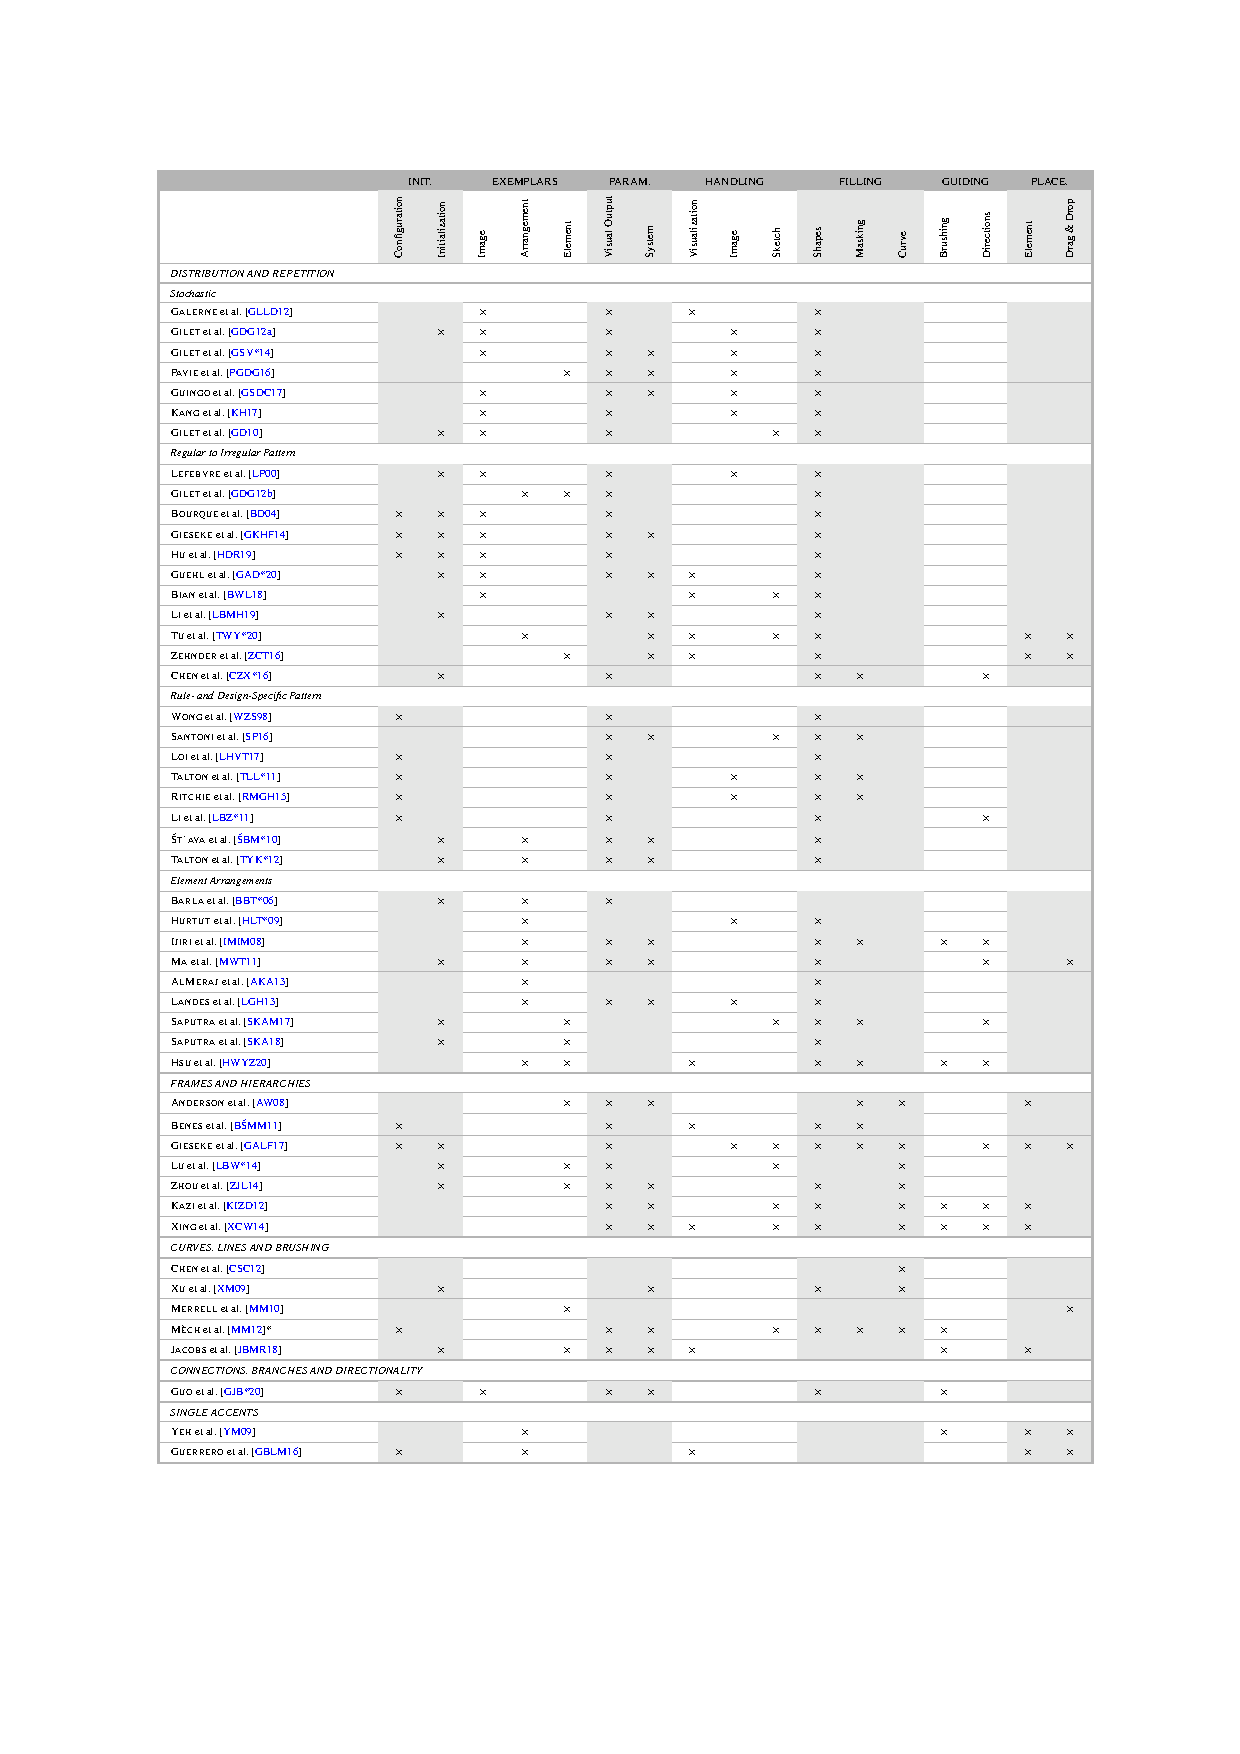
\includegraphics[width=0.9\textwidth]{tables/table_all.pdf}
%     \caption[Control mechanisms in the state of the art]{Recent techniques are sorted by design areas and visual features they enable. For each work it is analysed and indicated which specific control mechanisms they offer. *Please note that \cite{mech_2012_tdf} present a procedural modeling engine, which in principle can be programmed to include almost any control type.\label{table:analysis}}
% \end{table*}


\section{Discussion and Creative Means}
\label{sec:discussion_creative_means}

% TODO: More discussion for table:analysis
Table~\ref{table:analysis} lists for the above discussed publications the control mechanisms, which are categorized in~\Cref{sec:taxo_control_mechanism}. For interrelating the control mechanisms to the control characteristics, we considered the same publications in Table~\ref{table:taxo_controlmechanism}. Due to the diversity of the underlying methods and the different design goals of the considered body of work, we believe this to be a representative summarization.

Table~\ref{table:taxo_controlmechanism} shows that global, hence automatic, control is usually enabled through intermediate representations, such as an example image, while on the other end of the spectrum, the placement of elements as part of the actual output is local, and automation is lost. Parameterization and the different types of handling also require abstracted input from an artist, such as the use of a slider. Sketch-based controls, such as an eraser, move the interaction onto the canvas and can make small-scale adjustments. The definition of a space or a curve to fill and masking areas is also usually done directly on the canvas but only influence the output indirectly. A brushing mechanism simultaneously creates the output directly on the canvas but can only do so in a limited region depending on the brush size, unless used to brush intermediate control lines. All other inputs are typically given before or after the generation of the output. The classification underlines that a focus on one control type, as is often done in computer graphics research, leads to the common trade-off between global automation and local manual manufacturing.

% TABLE
% This is for overaleaf a preview image as the table does not compile there...
\subimport{tables/}{table_controlmechanism}

% \begin{table}
%     \centering
%     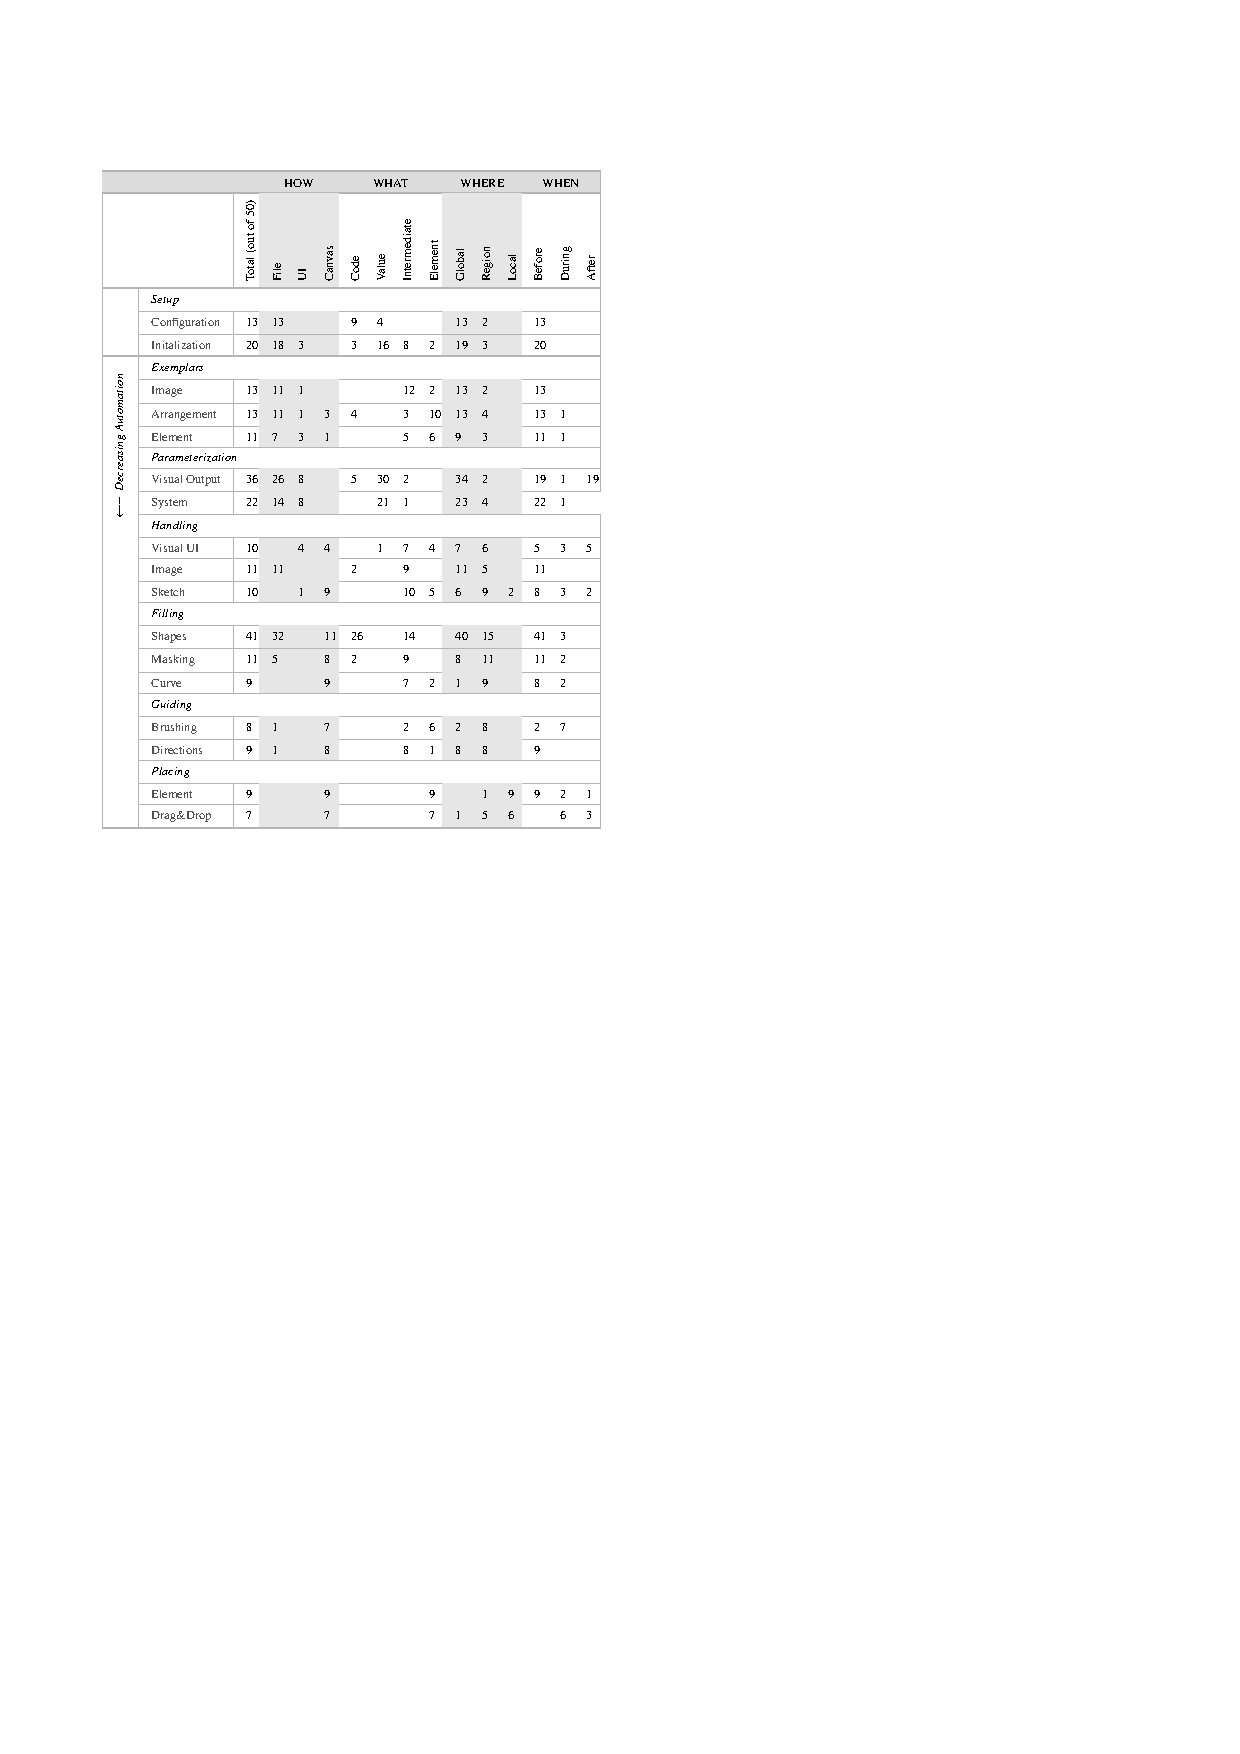
\includegraphics[width=\linewidth]{tables/table_controlmechanism.pdf}
%     \caption[Prevalence of control mechanisms]{Prevalence of control mechanisms in the literature: In total, 50 publications are included (the discussed state of the art work). Please note, that the totals of each step (how, what, where, when) can exceed the total of that category as it can be implemented within multiple usage scenarios.\label{table:taxo_controlmechanism}}
% \end{table}

We now discuss the techniques' potential to support a creative workflow, clustered into the most common types of control. This discussion of the creative means has an interpretative nature to it. Arguably, not always is an unambiguous reasoning manageable. Thus, this discussion should be viewed as a step toward an objective discussion about terms such as artist-usable and creatively controllable as well as a more realistic usage of these terms.

\subsection{Example-Based Control}
\label{subsubsec:analysis_creative_means_example}

As the state of the art shows, one of the most prominently investigated techniques for texturing methods are example-based and inverse approaches. Example-based control mechanisms provide a \textit{goal-oriented control}. The motivation behind using these techniques is mainly to generate a specific and predictable output as efficiently as possible. This type of control stands in contrast to exploration. Example-based approaches detach the design task to a data-driven image generation technique, such as taking a photograph or designing a sample in an application such as Adobe Photoshop or Illustrator. Relevant factors for differentiating example-based techniques are the size of the design space, hence their expressiveness, performance and initialization requirements. 

The investigation of example-based techniques shows valuable achievements for goal-oriented control and for increasing design spaces within specific contexts. With regard to creative control, in addition to the gain in variability being a crucial step, the presented work also improves navigability through interactive performances. However, many techniques still require considerable non-creative effort for an artist, such as working with a power spectrum or predicting how changes in the exemplar, such as element arrangements, affect the output. \citeauthor*{tu_2020_cct}~\cite{tu_2020_cct} and \citeauthor*{bian_2018_tpd}~\cite{bian_2018_tpd} combine the drawing of a tile with an automatic tiling system, a promising direction, as it offers transparent navigation. Also, through the drawing of the tiles the design space is fairly open within the scope of the specific pattern type, which is further limited by fabrication constraints in case of \citeauthor*{bian_2018_tpd}~\cite{bian_2018_tpd}. Both techniques offer support for the artist directly on the canvas such as editing options on the tiling itself~\cite{tu_2020_cct}, as well as preview and snapping functionalities making it easy for an artist to create structurally sound patterns~\cite{bian_2018_tpd}. 

The potential of example-based methods for creative control lies in furthering interactive performance, reducing initialization requirements and experimenting with the spatial influence of the input, such as introduced by \citeauthor*{guehl_2020_stu}~\cite{guehl_2020_stu} with a semi-procedural generation of stochastic textures. Overall, the presented work focuses on global designs, such as the whole canvas and repeating regions. Methods for which regions could be defined, models layered or the placement of single elements integrated constitute valuable directions for example-based methods as creative control.


\subsection{Shapes and Masks}
\label{subsubsec:analysis_creative_means_shapes}

Sophisticated masks and growth constraints lead to visually interesting and complex designs, such as the packing pattern from~\citeauthor*{saputra_2018_rde}~\cite{saputra_2018_rde}. However, it is not directly predictable how a space will be filled exactly. Because many of the presented methods only offer quite limited interactive performance, even a basic trial and error exploration is hardly feasible; hence, the navigation of the design space becomes cumbersome, and stimulation becomes hindered. The one technique \cite{santoni_2016_ggp} that offers the means for a transparent navigation is also the one with a fairly harsh restricted design space. \citeauthor*{santoni_2016_ggp}~\cite{santoni_2016_ggp}s' consideration of a navigation history stands out from the related work in this survey. In terms of stimuli, the mass-spring system for editing control guides offered by \citeauthor*{benes_2011_gpm}~\cite{benes_2011_gpm}, as well as the elastic curves from \citeauthor*{zehnder_2016_dso}~\cite{zehnder_2016_dso} are promising directions because they are intuitive and enjoyable to use and encourage exploration.

In terms of control mechanisms for a more complex design goal, shape fillings and masks do not permit hierarchical or element-level local controls or the control of element connections needed by artists who want to generate patterns creatively without having to write code.


\subsection{Vector Fields}
\label{subsubsec:analysis_creative_means_fields}

Fields (in the context of this survey usually vector fields) constitute a powerful tool for combining an automatic procedural filling by individually designing regions on the canvas. As \citeauthor*{hsu_2020_aef}~\cite{hsu_2020_aef}, ~\citeauthor*{saputra_2017_ffo}~\cite{saputra_2017_ffo} and \citeauthor*{gieseke_2017_ooo}~\cite{gieseke_2017_ooo} show, the streamlines of a field can create curves as part of the pattern that fill and structure a space. The design of a vector field requires usually less manual work to fill a space in its entirety by inputing only a few curves that control, \eg~directionality, than the manual creation, \eg~drawing of all curves needed for the filling. Other global design choices, such as an overall growth direction or the alignment of elements, are simple to translate from a vector field to procedural generation rules.

The discussed work shows that fields allow for greater visual variation by opening the design space and transparent control for filling a space automatically. When designing a vector field, artists do not work with the pattern directly, but fields are intuitive to understand. Their abstraction translates to the model in a straightforward manner. Thus, using flow within a vector field to design is a suitable control mechanism, especially for designs that aims to align their elements to the space.

\subsection{Curves and Brushing}
\label{subsubsec:analysis_creative_means_curves}

Curves and hand-drawn paths give an artist direct control over the final result. In addition to the visual output being further constrained, the control is put onto the actual canvas. Curves are needed for tasks such as creating a decorative frame or structuring the space. Some techniques consider the whole curve before computing the pattern, optimizing the filling of the curve based on certain design goals, enabling a form of global planning.

Curves and sketch-like methods offer a well communicated, hence transparent navigation. The discussed techniques are mostly interactive, artists are familiar with their functionality from the real world and they work directly on the canvas. The ease and directness of usage also constitute a foundation for possible immersive flow of work. Using painting-like methods can allow for smoother navigation by integrating brush settings and increasing the quantity of controls.

However, because creation techniques and design spaces are open, it could lead to manual and tedious creation requirements for patterns. To balance this \citeauthor*{kazi_2012_vit}~\cite{kazi_2012_vit} and \citeauthor*{xing_2014_apr}~\cite{xing_2014_apr} incorporate procedural creation principles for automatic fillings into a data-driven process. \citeauthor*{hsu_2020_aef}~\cite{hsu_2020_aef} offer through a brushing system transparent navigation and an open design space within the topic of element arrangements. With a brush an artist is free to draw almost anything - depending only on one's personal drawing capabilities. For creative pattern generation elements are often carefully connected, creating a hierarchy of structures, such as for ornaments. Hence, element arrangements can only provide a subset - albeit an important one - of the design space needed for creative pattern generation. 

\subsection{Element Placement}
\label{subsubsec:analysis_creative_means_elements}

The placement of single elements onto the canvas maximizes artist control and is on its own a trivial data-driven control principle. However, in combination with procedural modeling, this mechanism becomes interesting. Separately placed elements that do not follow any rules should be integrated and processed to remain part of the underlying global scene structure, as demonstrated by \citeauthor*{gieseke_2017_ooo}~\cite{gieseke_2017_ooo}. Even though single element placements can be compared to using the tip of a brush, paint-like procedural modeling techniques often have a more spray-can-like quality, such as \citeauthor*{hsu_2020_aef}~\cite{hsu_2020_aef} and \citeauthor*{mech_2012_tdf}~\cite{mech_2012_tdf}. Element placement control mechanisms are closely related to the data-driven sketch-based techniques, and it shows a further promising approach for integrating procedural modeling functionalities into a data-driven process. \citeauthor*{guerrero_2016_pep}~\cite{guerrero_2016_pep} present a overall transparently navigable and stimulating control mechanism. With a carefully designed workflow, it further fosters an artist stimulation by offering novel but suitable design variations.

